\chapter{ANÁLISE DOS RESULTADOS DA  PESQUISA}
\label{chap:analise}

Segundo \citeonline{poltronieri2018usability}, há muito esforço para criar e usar \gls{DSL}s como recurso de facilitar a construção do sistema, aumentar a produtividade e facilitar a manutenção. No entanto, as \gls{DSL}s tratam do problema de domínio (usuários especialistas) e não somente do domínio de solução (desenvolvedores/engenheiros de software), isso significa que nem sempre há aceitação e entendimento entre esses usuários.

Nesse sentido, este Capítulo apresenta a análise dos dados obtidos em relação aos 2 (dois) instrumentos de coleta de dados (exercício de avaliação da DSL Cotas e o questionário aplicado com usuários), bem como, os resultados com os testes da API DSL Cotas. Esses instrumentos têm como foco verificar se a DSL Cotas atinge seus objetivos em relação à perspectiva dos diferentes grupos de usuários. 

Para melhor sistematizar a organização dos dados optou-se por apresentar a análise por grupos de usuários, considerando os diferentes perfis de experiência, os resultados foram agrupados de acordo com os 4 (quatro) grupos:  DEV-NESP; DEV-ESP; NDEV-ESP e NDEV-NESP, cujos perfis são definidos na Seção \ref{sec:idperfis}. Na Seção \ref{sec:perguntasaplicadas} são apresentados os dados gerais sobre as perguntas aplicadas com os usuários, enquanto a Seção \ref{sec:analiseexercicio} expõe os resultados obtidos com o exercício prático proposto aos usuários convidados, os resultados obtidos com a aplicação do questionário após a realização do exercício e algumas mudanças aplicadas na DSL Cotas com base nas sugestões dos usuários. Por fim, a Seção \ref{sec:avaliacaoapi} detalha os resultados dos testes com a API.





\section{Identificação dos perfis de usuários}
\label{sec:idperfis}


A Figura \ref{fig:perfilusuarios} apresenta o perfil de cada usuário que participou da avaliação de uso da DSL Cotas. Os critérios para inserção em cada grupo são descritos a seguir:

\begin{enumerate}
    \item[a)] \texttt{DEV-ESP}: usuários que possuem conhecimento sobre a lei nº 12.711 e suas atualizações, são desenvolvedores e já atuaram em sistemas ou processos seletivos que utilizam o sistema de cotas;
    \item[b)] \texttt{DEV-NESP}: usuários com perfil de desenvolvedor sem conhecimento ou com conhecimento restrito sobre a legislação;
    \item[c)] \texttt{NDEV-ESP}: usuários com conhecimento na legislação, não desenvolvedores. Em sua maioria usuários que trabalham em setores que organizam processos seletivos relacionados ao sistema de cotas;
    \item[d)] \texttt{NDEV-NESP}: usuários não conhecedores da legislação e não desenvolvedores, de modo que pudesse ser identificado se as pessoas com esse perfil teriam dificuldades com a utilização da linguagem.
\end{enumerate}


\begin{landscape}
\begin{figure}[ht!]
\centering

\caption{\textmd{Perfil dos usuários participantes}}
\label{fig:perfilusuarios}
\fcolorbox{gray}{white}{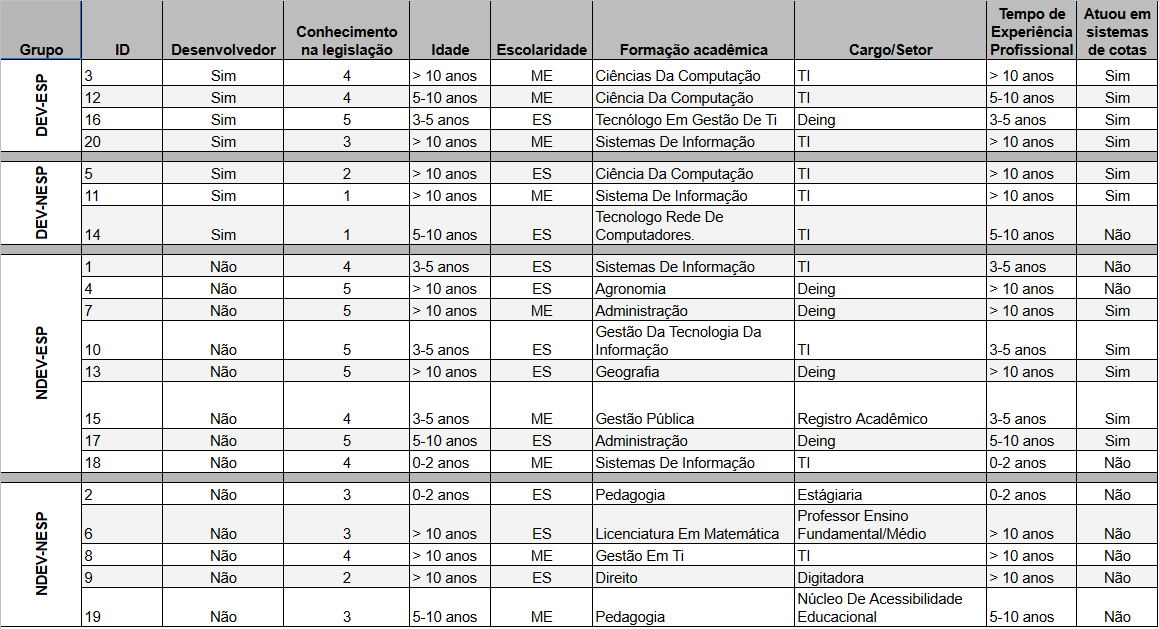
\includegraphics[width=1.5\textwidth]{chapters/analise/imagens/perfilusuarios.png}}

\par\medskip\textbf{Fonte:} Elaboração do autor (2020). \par\medskip

\end{figure}

\end{landscape}

\section{Informações obtidas com o questionário}
\label{sec:perguntasaplicadas}

Esta seção apresenta as perguntas do formulário \textit{on-line} submetido para todos os usuários participantes do presente estudo. As perguntas foram aplicadas após o término da execução do exercício, buscando obter as informações necessárias para cada perfil de usuário da DSL, assim como, entender as principais dificuldades encontradas por eles na utilização da linguagem.

As 5 (cinco) primeiras perguntas tem como objetivo levantar dados demográficos, tais como: nível de formação escolar, curso de formação acadêmica, cargo, tempo de experiência profissional e a informação se elas possuem experiência com desenvolvimento de sistemas.

O formulário \textit{on-line} recebeu 20 respostas, das quais contou com a representatividade de profissionais da área de tecnologia da informação (50\%) e profissionais atuantes em setor de ingresso de estudantes (20\%), além de outros setores como pode ser observado no gráfico da Figura \ref{fig:experienciacargo}. Desses profissionais, 68,4\% indicaram não ter experiência prévia com desenvolvimento de sistemas, enquanto, 31,6\% informaram já terem experiência de desenvolvimento.

\begin{figure}[ht!]
\centering

\caption{\textmd{Cargo e experiência de desenvolvimento}}
\label{fig:experienciacargo}
\fcolorbox{gray}{white}{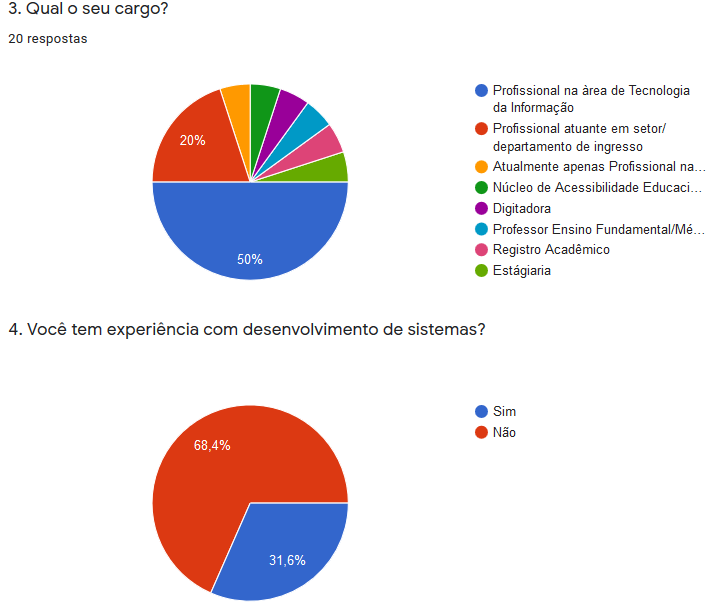
\includegraphics[width=0.80\textwidth]{chapters/analise/imagens/experienciacargo.png}}

\par\medskip\textbf{Fonte:} Elaborada pelo autor (2020). \par\medskip

\end{figure}



\newpage
Para levantar o conhecimento e a experiência sobre o sistema de cotas da rede de ensino federal foram submetidas as seguintes perguntas: "6. Você já atuou em sistemas ou processos seletivos que utilizam regras de classificação para candidatos cotistas?" e "7. Qual o seu grau de conhecimento sobre o sistema de cotas da Lei nº 12.711/2012 e suas atualizações?" (Figura \ref{fig:grauconhecimento}).

\begin{figure}[ht!]
\centering

\caption{\textmd{Perfil de conhecimento e atuação em processos}}
\label{fig:grauconhecimento}
\fcolorbox{gray}{white}{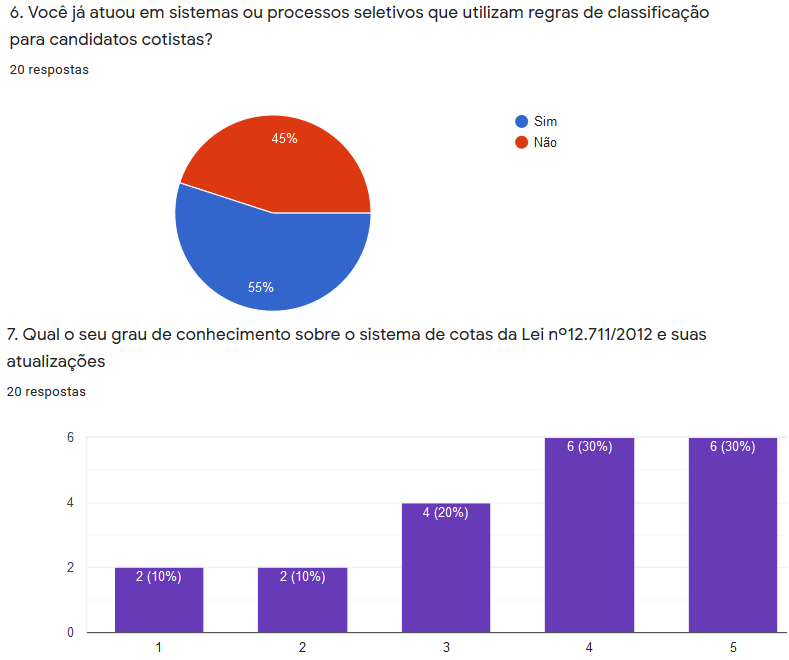
\includegraphics[width=0.85\textwidth]{chapters/analise/imagens/grauconhecimento.png}}

\par\medskip\textbf{Fonte:} Elaborada pelo autor (2020). \par\medskip

\end{figure}



Com o intuito de identificar se os usuários já tiveram contato com outras DSLs, a pergunta "8. Você já utilizou alguma Linguagem de Domínio Específica? Exemplos: HTML, Excel, Latex, SQL, etc.", mostrou que 55\% dos usuários já tiveram contato com outras aplicações ou softwares que utilizam alguma \gls{DSL}, enquanto os demais apontaram não conhecer nenhuma DSL (Figura \ref{fig:usodsl}).

\begin{figure}[ht!]
\centering

\caption{\textmd{Experiência prévia com DSLs}}
\label{fig:usodsl}
\fcolorbox{gray}{white}{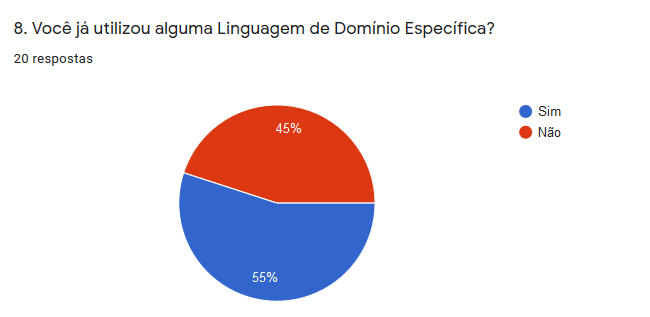
\includegraphics[width=\textwidth]{chapters/analise/imagens/usodsl.png}}

\par\medskip\textbf{Fonte:} Elaborada pelo autor (2020). \par\medskip

\end{figure}



\newpage
Em continuidade, foram adicionadas as seguintes perguntas responsáveis pelo levantamento de dificuldades de uso com a DSL:

\begin{enumerate}

    \item[a)] 9. De modo geral, qual o grau de dificuldade para execução do exercício proposto?;
    
    \item[b)] 10. Considerando a sua resposta na pergunta anterior, qual(is) a(s) dificuldade(s) encontrada(s)?;
    
    \item[c)] 11. Na sua avaliação quais as principais limitações da linguagem proposta?;
    
   \item[d)]  12. Quais dos materiais abaixo você utilizou para execução do exercício?;
   
   \item[e)] 13. No caso de a linguagem apresentar erros "destaques em vermelho" ou avisos "destaques em amarelo", as mensagens foram claras e ajudaram a resolver o(s) problema(s) apresentado(s)?;
   
   \item[f)] 14. Quanto tempo, aproximadamente, você utilizou para executar o exercício proposto?.   

\end{enumerate}

Em linhas gerais, o grau de dificuldade de uso da DSL, em escala de 1 (difícil) e 5 (fácil), pode ser observado na Figura \ref{fig:dificuldadegeral}. O formulário completo foi disponibilizado no (APÊNDICE \ref{chap:apen:formularioapen}). 

\begin{figure}[ht!]
\centering

\caption{\textmd{Dificuldade de uso e deficiências da DSL}}
\label{fig:dificuldadegeral}
\fcolorbox{gray}{white}{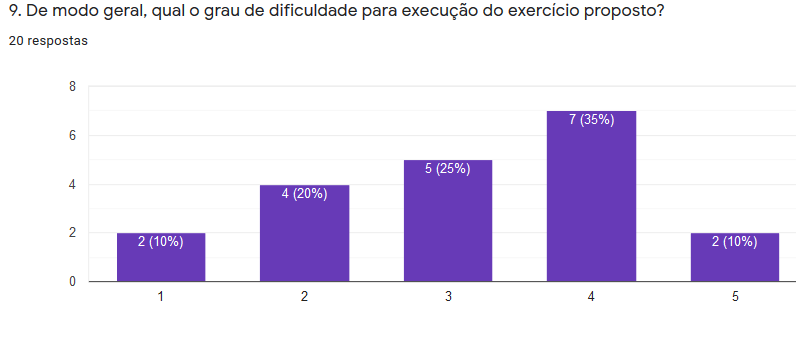
\includegraphics[width=0.85\textwidth]{chapters/analise/imagens/dificuldadegeral.png}}

\par\medskip\textbf{Fonte:} Elaborada pelo autor (2020). \par\medskip

\end{figure}



\newpage
Os demais resultados obtidos com o formulário e os exercícios são descritos com maiores detalhes nas próximas Seções.




\section{Resultados obtidos com o exercício}
\label{sec:analiseexercicio}

Cada usuário recebeu por e-mail um manual  contendo as principais instruções para uso da DSL Cotas, incluindo conceitos sobre cada elemento da legislação. Adicionalmente, a esse manual foi definido um exercício aberto, no qual, a tarefa proposta é definir os requisitos da primeira versão da lei nº 12.711 (Figura \ref{fig:exercicio}). 

\begin{figure}[ht!]
\centering

\caption{\textmd{Versão proposta para exercício da DSL}}
\label{fig:exercicio}
\fcolorbox{gray}{white}{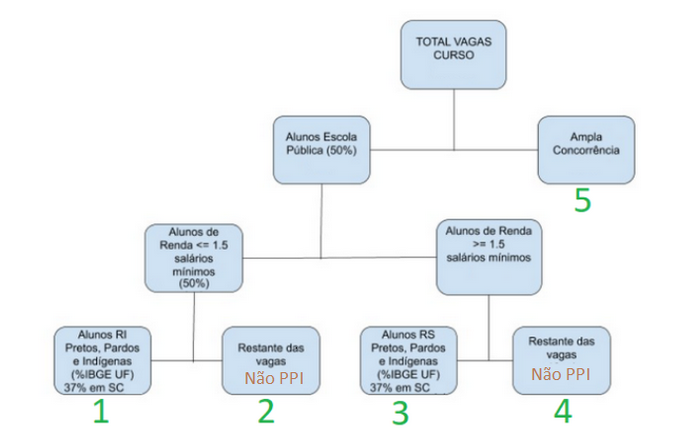
\includegraphics[width=0.85\textwidth]{chapters/analise/imagens/exercicio.png}}

\par\medskip\textbf{Fonte:} Elaboração do autor (2020). \par\medskip

\end{figure}



Essa versão foi escolhida por ser mais simples se comparada as versões mais recentes, requerendo um tempo menor de dedicação ao exercício e adequando a complexidade para todos os grupos dos diferentes perfis de usuários. 


Com o intuito de avaliar o exercício, todas as 20 respostas foram salvas imediatamente após o término no sistema de controle de versão \texttt{git}. Cada resposta foi salva em um \texttt{branch} disponível no repositório \texttt{https://github.com/spgroup/dsl-cotas/branches}.


Durante essa análise foram contabilizados os acertos em relação aos seguintes elementos da linguagem: distribuição de vagas (níveis e categorias criadas), configurações de percentuais (definição e utilização durante a distribuição), definição completa da ordem de prioridade (ordem indicada e quantidade de categorias presentes), quantidade de \textit{errors} e \textit{warnings} não resolvidos, e a presença de versão da legislação mais recente implementada opcionalmente por alguns usuários.

A seguir são apresentados os resultados da aplicação do exercício para cada grupo.


\subsection{Resultados do Grupo DEV-ESP}
\label{subsec:devesp}

Em relação à pergunta "9. De modo geral, qual o grau de dificuldade para execução do exercício proposto?", em uma escala de 0(difícil) e 5(fácil), nesse grupo de usuários todos indicaram a nota 4 e 5. Ademais, foram realizadas as seguintes considerações:

\begin{enumerate}
    \item [a)] "Dúvidas de primeiro uso, do tipo -o que  mesmo que eu devia digitar maiúsculo?-, -será que preciso mesmo digitar 50.0 ou só 50?-,  entre outras do gênero. Como é execução de um exercício que é feito pela primeira vez, esse tipo de dúvida acaba não deixando totalmente fácil, pois eventualmente é necessário rever alguma instrução. Mas de resto, se já tiver esses detalhes na cabeça, a execução seria bem fácil (Usuário 20).";
    
    \item[b)] "A sequência de prioridades final onde se define quais candidatos se seleciona primeiro, foi um pouco mais difícil fazer a seleção... A dificuldade do último item pode ser melhorada com implementação ou instruções. No mais ficou bem interessante para configurar a árvore de decisão e percentuais aplicados (Usuário 3).".
\end{enumerate}

Conforme relatado pelo Usuário 20, no primeiro contato com a DSL surgem algumas dúvidas sobre o formato de preenchimento dos percentuais e de siglas de categorias, o que pode levar a necessidade de reescrita de algumas instruções da linguagem. De modo geral, isso pode ser resolvido a medida que se acostuma com a linguagem.

Outro aspecto levantado pelo Usuário 3 relaciona-se com problemas durante a definição da ordem de prioridade, em que o comando de adição de novos itens na lista não estava claro o suficiente na linguagem, sendo necessário melhorar a usabilidade desse elemento.

Os exercícios foram finalizados entre 15 a 30 minutos, sendo que 2 (dois) desses usuários (Usuário 20 e 16) fizeram completamente a definição da árvore de distribuição, sem \textit{errors} ou \textit{warnings}. Os outros dois usuários (Usuário 3 e 12) não resolveram alguns erros e avisos da linguagem, um deles criou um nível a mais de distribuição, gerando uma árvore de distribuição incorreta (Figura \ref{fig:errodevesp}). 

\begin{figure}[ht!]
\centering

\caption{\textmd{Exercício com erro na árvore de distribuição}}
\label{fig:errodevesp}
\fcolorbox{gray}{white}{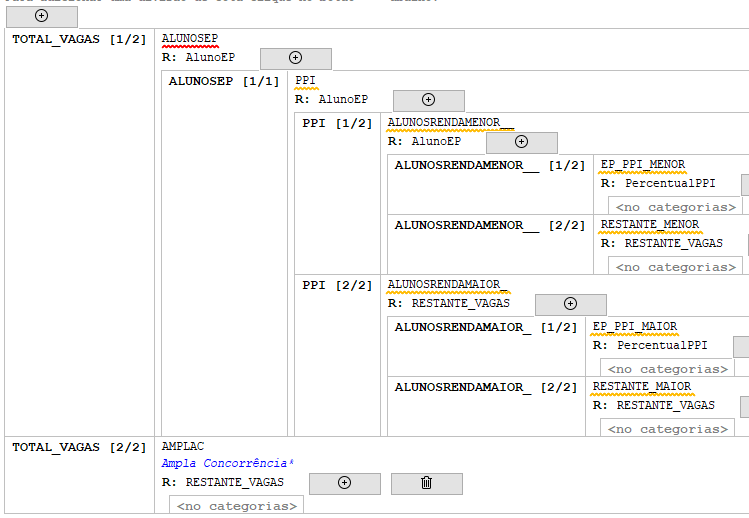
\includegraphics[width=0.85\textwidth]{chapters/analise/imagens/figerrodevesp.png}}

\par\medskip\textbf{Fonte:} Dados da pesquisa (2020). \par\medskip

\end{figure}






Com relação às respostas presentes na questão "11. Na sua avaliação quais as principais limitações da linguagem proposta?", 2 (dois) usuários informaram que: "As sugestões das mensagens informativas não são claras o suficiente (Usuários 16 e 20)", o que pode ter levado aos problemas descritos anteriormente.

Em relação a pergunta "13. No caso de a linguagem apresentar erros "destaques em vermelho" ou avisos "destaques em amarelo", as mensagens foram claras e ajudaram a resolver o(s) problema(s) apresentado(s)?", esse grupo indicou conseguir de maneira geral resolver os problemas tendo como base as mensagens apresentadas pela DSL, todos indicaram a pontuação de escala 4 e 5 (quatro e cinco), considerando a escala de 1(difícil) e 5(fácil).

Contudo, após o levantamento apresentado na Figura \ref{fig:quadro:grupodevesp}, foi possível identificar que os demais recursos e percentuais foram preenchidos corretamente. Destaca-se que o grupo em análise, possui bom conhecimento na área de domínio, além de ter familiaridade com ferramentas de desenvolvimento e outras \gls{DSL}s, o que pode ter sido preponderante para que tenham indicado que a linguagem foi de fácil uso e entendimento. 
\begin{figure}[ht!]
\centering

\caption{\textmd{Quadro da análise do grupo DEV-ESP}}
\label{fig:quadro:grupodevesp}
\fcolorbox{gray}{white}{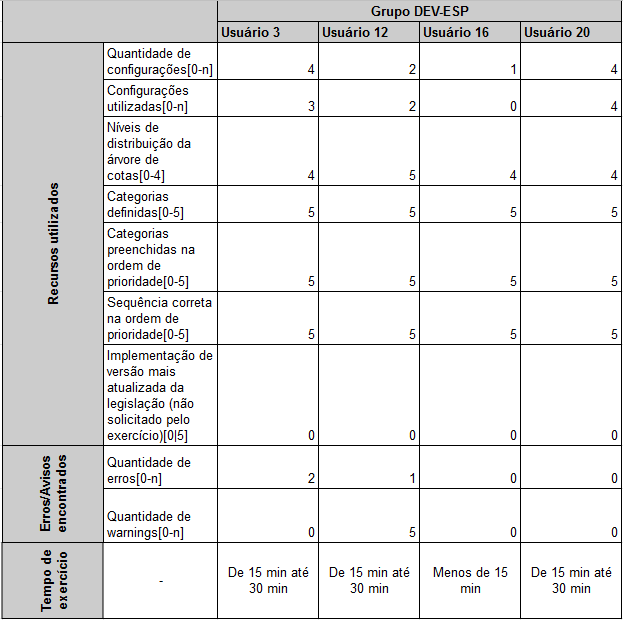
\includegraphics[width=0.85\textwidth]{chapters/analise/imagens/grupodevesp.png}}

\par\medskip\textbf{Fonte:} Elaboração do autor (2020). \par\medskip

\end{figure}


\newpage
\subsection{Resultados do Grupo DEV-NESP}
\label{subsec:devnesp}

Nesse grupo, com relação à pergunta sobre o grau de dificuldade, os usuários apontaram os níveis 2 e 3 (três e dois), considerando a escala de 1(difícil) e 5(fácil). No exercício do Usuário 6 constaram vários erros não resolvidos na distribuição de vagas, em sua maioria em relação ao padrão de nomenclatura das siglas das categorias de cotas (Figura \ref{fig:errodevnesp}). 

\begin{figure}[ht!]
\centering

\caption{\textmd{Exercício do Usuário 11}}
\label{fig:errodevnesp}
\fcolorbox{gray}{white}{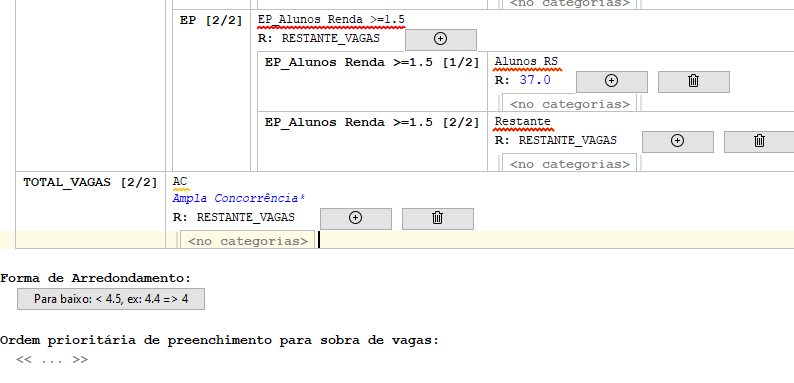
\includegraphics[width=0.85\textwidth]{chapters/analise/imagens/figerrodevnesp.png}}

\par\medskip\textbf{Fonte:} Elaboração do autor (2020). \par\medskip

\end{figure}



\newpage


Adicionalmente à questão sobre o grau de dificuldade foram feitos os seguintes comentários:

\begin{enumerate}
    \item [a)] "Foi difícil entender o funcionamento do sistema (Usuário 5)";
    \item [b)] "No exercício não compreendi se era pra utilizar a a ordem de prioridade ou não, se segue o padrão de uma árvore ou teria que informar. A questão do arredondamento ficou um pouco confusa, depois que entendi que é apenas uma configuração caso utilizar números quebrados nos percentuais (Usuário 11)";
    \item [c)] "Tive dificuldade em entender a proposta por não conhecer a lei específica.  (Usuário 14)".    
\end{enumerate}

Portanto, nota-se a dificuldade de entendimento de questões relacionadas à legislação do sistema de cotas e, adicionalmente, algumas dificuldades sobre uso do elemento de ordem de prioridade da linguagem. 

Em continuidade a essa análise, apresentam-se as considerações para a pergunta que trata sobre as limitações da linguagem: "Não observei a execução de uma emulação de processo em prática (Usuário 5)", "As sugestões das mensagens informativas não são claras o suficiente (Usuário 11)".

Considerando a limitação apontada pelo Usuário 5, observa-se a falta do \textit{feedback} por parte da DSL para simulação da distribuição de vagas, uma vez que a função responsável por fazer os cálculos do quadro de vagas foi implementada apenas na API DSL Cotas. 

Novamente foram apontados problemas nas mensagens geradas pela linguagem, conforme relato do Usuário 11. Esse usuário afirma que: "O vídeo didático poderia ser mais alto e com mais instruções de utilização.", indicando que são necessárias mais instruções no manual e no vídeo explicativo para conseguir melhorar o entendimento da linguagem. 

Ademais, as seguintes sugestões foram levantadas por meio da pergunta número 15 do questionário:

\begin{citacao}
A linguagem auxilia a documentar o processo. Acredito que ela implemente a execução da coleta de dados. Espero que ela saiba ler os dados de várias bases diferentes, e não exija um tratamento nestes dados muito extenso, senão é talvez mais viável inserir diretamente os dados em uma base relacional e executar as ordenações necessárias (Usuário 5).
\end{citacao}

Tendo em vista os apontamentos descritos para o grupo, observa-se que a falta de entendimento nas regras de domínio dificulta o uso da linguagem (Usuários 11 e 14), no entanto, há maiores preocupações relacionadas à simulação e aos detalhes de implementação para o processamento final das regras (Usuário 5). Conforme o levantamento descrito na Figura \ref{fig:quadro:grupodevnesp},  observou-se um tempo maior para o exercício do Usuário 5 (Mais de 30min).

\begin{figure}[ht!]
\centering

\caption{\textmd{Quadro da análise do grupo DEV-NESP}}
\label{fig:quadro:grupodevnesp}
\fcolorbox{gray}{white}{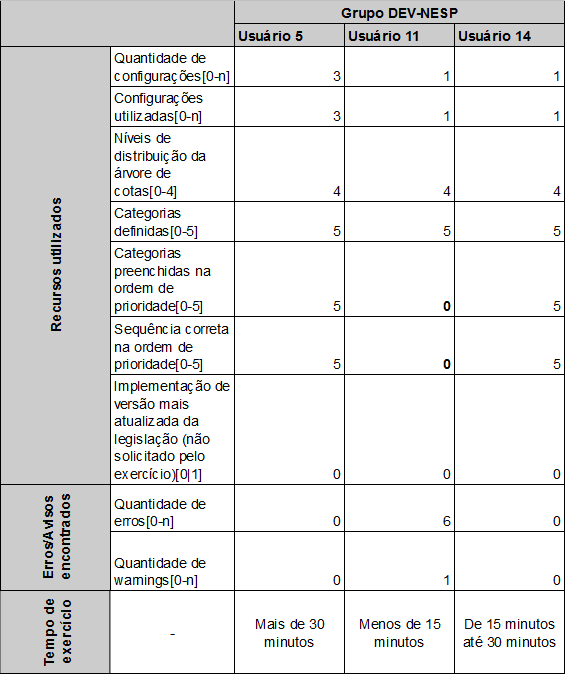
\includegraphics[width=0.77\textwidth]{chapters/analise/imagens/grupodevnesp.png}}

\par\medskip\textbf{Fonte:} Elaborada pelo autor (2020). \par\medskip

\end{figure}






\newpage
\subsection{Resultados do Grupo NDEV-ESP}
\label{subsec:ndevesp}

Nessa Subseção são analisados os dados dos participantes cujos perfis indicam maior proximidade com os usuários finais da DSL Cotas. Esses usuários, em sua maioria, já participaram da organização de processos seletivos com base no sistema de cotas, no entanto, não possuem nenhuma experiência com ferramentas de desenvolvimento de sistemas.

A Figura \ref{fig:dificuldadendevesp} demonstra o gráfico elaborado para as 8 (oito) respostas do grupo em relação à pergunta 11 do formulário, na qual em uma escala de 1 (difícil) a 5 (fácil) foi possível identificar que 50\% dos usuários tiveram maior facilidade (escala 4), 25\% indicaram a escala intermediária de dificuldade (escala 3) e os demais consideraram o uso da DSL como difícil (escalas 1 e 2). 

\begin{figure}[ht!]
\centering

\caption{\textmd{Gráfico de respostas com a escala de dificuldade}}
\label{fig:dificuldadendevesp}
\fcolorbox{gray}{white}{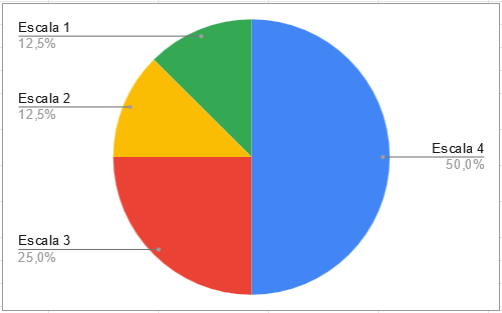
\includegraphics[width=0.85\textwidth]{chapters/analise/imagens/dificuldadendevesp.png}}

\par\medskip\textbf{Fonte:} Elaborado pelo autor (2020). \par\medskip

\end{figure}



Considerando os comentários dos usuários sobre essa pergunta, destacam-se as seguintes observações:

\begin{enumerate}
    \item [a)] "É necessário familiarizar-se com o ambiente proposto para o exercício.  (Usuário 1)";
    
    \item [b)] "Apenas dificuldade inicial para entender a lógica dos comandos. Logo após este entendimento, tornou-se fácil a utilização. O tutorial está muito claro, mas talvez um melhor suporte com menagens informativas no próprio ambiente, ao clicar nas etapas (Usuário 7)";
    
    \item [c)] "Primeiro momento parece simples, mas como preencher corretamente, as siglas finais, fiquei um pouco confusa, e ao preencher um percentual no próximo só dar ctrl + backspace ou somente colocar RESTANTE\_VAGAS... No final da ordem de como vai ser preenchido os restantes de vaga precisava ser um pouco mais claro, .. no geral é uma ótima ferramenta, mas necessitaria mais algumas aulas para ficar fera (Usuário 10)";
    
    \item [d)] "Demorei um pouco para entender o funcionamento, a regra do sistema, mesmo após ver o vídeo explicativo. Após isso, interpretar a lei, ou o exercício, e aplicar no sistema também surtiu uma certa dificuldade - refiz 3 vezes até entender que estava de acordo com o proposto (Usuário 13)";
    
    \item[e)] "O preenchimento na distribuição de vagas, sendo o entendimento do funcionamento das regras, após ter uma dificuldade com a variável pré existente de RESTANTE\_VAGAS, e a relação com as configurações acima, o procedimento ficou mais claro (Usuário 18)".
\end{enumerate}

Portanto, observa-se que esse grupo teve dificuldades relacionadas ao uso de comandos e regras da DSL, no que concerne à etapa de distribuição de vagas. Todos os usuários citados relatam que essas dificuldades foram resolvidas após algum tempo de uso da DSL Cotas.

Destaca-se que, 2 (dois) usuários do grupo (Usuário 4 e 7), implementaram a versão mais atualizada da legislação, na qual é composta de 5(cinco) níveis de distribuição e 9 (nove) categorias, incluindo a subdivisão para candidatos PCD (Figura \ref{fig:ndevesp}). Essa versão não foi proposta pelo exercício e, mesmo assim, esses usuários avançaram na utilização da DSL Cotas opcionalmente. Isso pode indicar que, apesar das dificuldades encontradas, foi possível utilizar a DSL Cotas até para situações mais complexas não previstas pelo exercício.


\begin{figure}[ht!]
\centering

\caption{\textmd{Exercício com a versão atualizada da lei}}
\label{fig:ndevesp}
\fcolorbox{gray}{white}{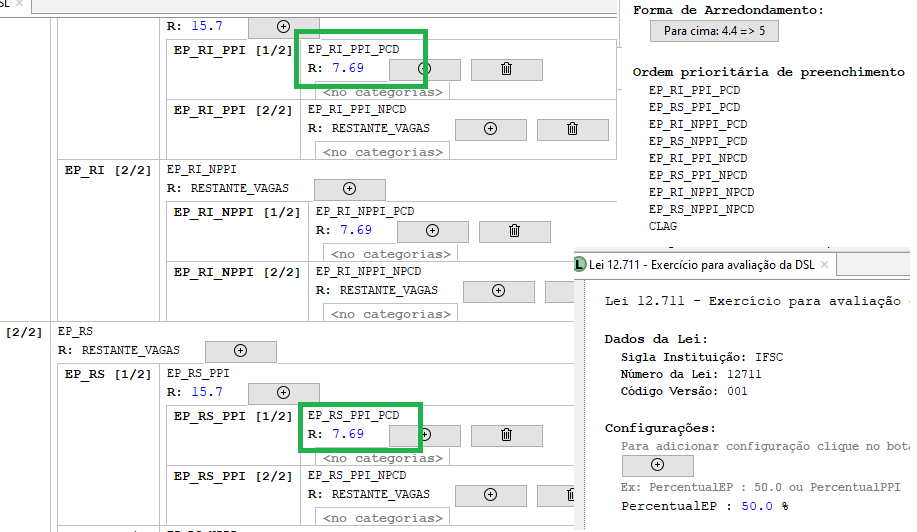
\includegraphics[width=\textwidth]{chapters/analise/imagens/figndevesp.png}}

\par\medskip\textbf{Fonte:} Dados da pesquisa (2020). \par\medskip

\end{figure}



Nesse grupo, o Usuário 4 levou mais de 1 (uma) hora para fazer a implementação do exercício, embora este também tenha utilizado a versão mais recente como base para descrição na DSL Cotas. Os demais, em sua maioria, conseguiram finalizar o exercício entre 15 e 30 minutos (Figura \ref{fig:quadro:grupondevesp}).

\begin{figure}[ht!]
\centering

\caption{\textmd{Quadro da análise do grupo NDEV-ESP}}
\label{fig:quadro:grupondevesp}
\fcolorbox{gray}{white}{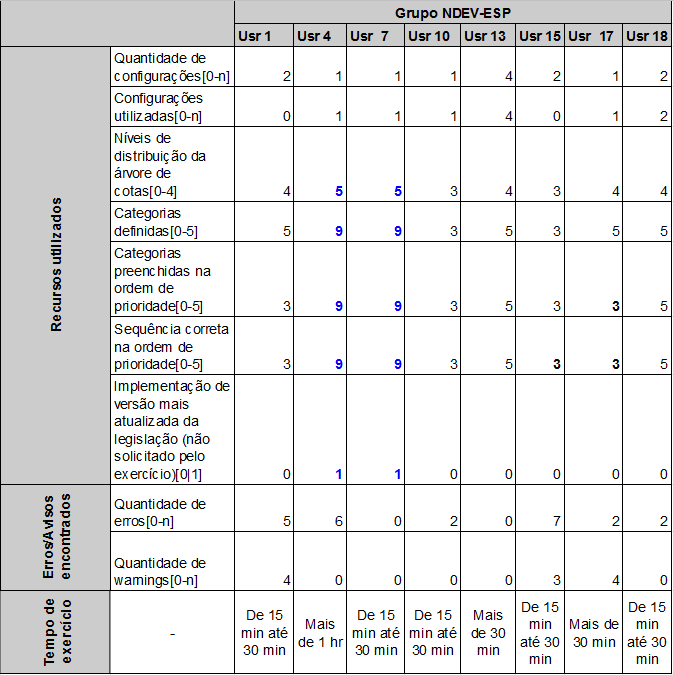
\includegraphics[width=0.85\textwidth]{chapters/analise/imagens/grupondevesp.png}}

\par\medskip\textbf{Fonte:} Elaboração do autor (2020). \par\medskip

\end{figure}



Sobre a pergunta "11. Na sua avaliação quais as principais limitações da linguagem proposta?", 4 (quatro) usuários apontaram que a principal limitação é: "As sugestões das mensagens informativas não são claras o suficiente". O Usuário 13 relatou que "O layout talvez não seja tão amigável para leigos em programação, o que dificulta um pouco para identificar onde clicar e o que digitar".

Assim como nos demais grupos de usuários, o grupo NDEV-ESP sugere melhorias nas mensagens informativas e na apresentação dos elementos da linguagem. Adicionalmente, algumas considerações foram observadas após análise do questionamento número "15. Comentários e Sugestões":

\begin{enumerate}
    \item [a)] "A fim de evitar erros e facilitar a compreensão, o sistema poderia apresentar, ao operador, uma simulação da distribuição de vagas para cada cota. Ex: Inicialmente o sistema mostra na variável RESTANTE\_VAGAS o valor 100 (ou outro valor). Após inserida a cota de ampla concorrência (CLAG) com percentagem de 50\%, a variável RESTANTE\_VAGAS apresenta o valor 50 e a CLAG apresenta o valor 50. E assim para todas as outras cotas. Ao final, seriam apresentadas as quantitativos de vagas para cada uma das cotas conforme os quadros dos editais de ingresso. (Usuário 1)";
    \item [b)] "O ambiente parece bastante prático e dinâmico, com facilidade de adaptação às necessidades de cada tipo de processo seletivo. (Usuário 7)";    
    \item [c)] "O manual de instruções está bem explicado, porém, por ser uma linguagem nova, pode haver dificuldade na interpretação das instruções, como foi meu caso. Confundi algumas instruções simples pois fiquei focado tentando entender os demais comandos que não conhecia. Porém, saliento que após utilizar a primeira vez, o sistema é de fácil manuseio. (Usuário 17)";   
    \item [d)] "Não tem um entendimento claro sobre as configurações de percentual. Ex: quando nas configurações eu preencho um percentual de PPI -  este é sobre o valor total ou sobre o valor da categoria que ele pertencer posteriormente. (Usuário 18)".
\end{enumerate}

Esses comentários rementem às sugestões de melhorias, tais como: a necessidade de simulação prévia da distribuição e maior clareza sobre o modo de configuração dos percentuais das categorias. Ademais, apesar de dificuldades na interpretação e uso dos comandos (Usuário 17), observou-se que há facilidade de adaptação às necessidades de cada tipo de processo seletivo (Usuário 7).

Por fim, considerando que os usuários do grupo conseguiram avançar no uso da DSL Cotas já no primeiro contato com a linguagem, mesmo sem ter conhecimento em desenvolvimento de sistemas, conclui-se que após terem maior familiaridade com a ferramenta, os usuários com domínio nas regras do sistema de cotas conseguem utilizar a DSL como meio de descrever as regras existentes na legislação.


\subsection{Resultados do Grupo NDEV-NESP}
\label{subsec:ndevnesp}

Diferentemente dos grupos de usuários desenvolvedores e especialistas, que são os principais envolvidos no processo de compreensão e implementação da legislação, o grupo NDEV-NESP foi escolhido para verificar se o design da DSL Cotas é simples o suficiente para pessoas leigas no assunto. Com isso, na medida em que sintam necessidade, consigam compreender mais facilmente o funcionamento das regras de cotas com o uso da DSL, seja por interesse próprio ou pelo fato de, por exemplo, precisarem atuar em setores ou ações institucionais que envolvam processos de classificação de candidatos.


Com relação ao levantamento da cursos da formação acadêmica do grupo foram informados os seguintes cursos: Pedagogia, Licenciatura em Matemática, Gestão em TI e Direito. Os dados levantados sobre o cargo atual dos usuários foram: Professor Ensino Fundamental/Médio, Estagiário, TI, Digitador e Profissional do Núcleo de Acessibilidade Educacional.

Em relação ao tempo de execução do exercício, esse grupo apresentou resultado variado. Os Usuários 6 e 19 levaram mais de 30 minutos, os Usuários 2 e 9 levaram de 15 até 30 minutos e o Usuário 8 levou menos de 15 minutos (Figura \ref{fig:quadro:grupondevnesp}). 

\begin{figure}[ht!]
\centering

\caption{\textmd{Quadro da análise do grupo NDEV-NESP}}
\label{fig:quadro:grupondevnesp}
\fcolorbox{gray}{white}{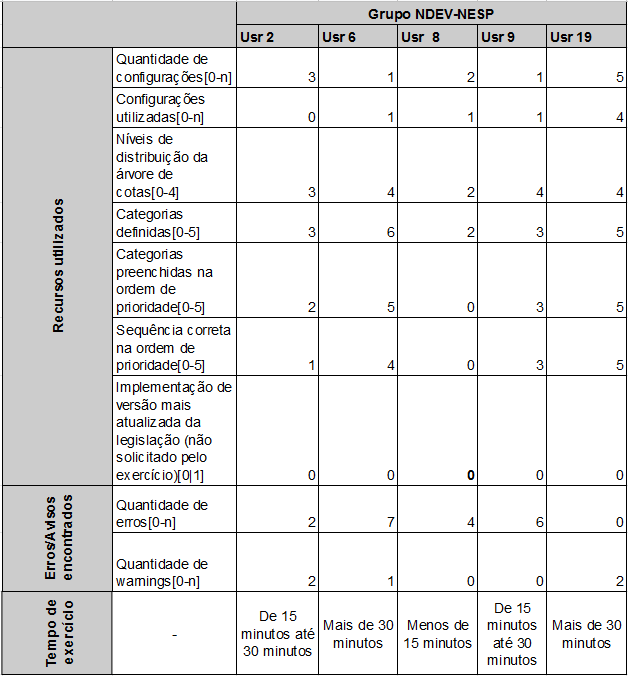
\includegraphics[width=0.80\textwidth]{chapters/analise/imagens/grupondevnesp.png}}

\par\medskip\textbf{Fonte:} Elaboração do autor (2020). \par\medskip

\end{figure}


\newpage

Após o levantamento, foi possível identificar que 3 (três) dos 5 (cinco) usuários, não implementaram corretamente a quantidade de níveis de distribuição proposta pelo exercício, os Usuários 2 e 8 implementaram, respectivamente, apenas 3 (três) e 2 (dois) níveis da árvore. O Usuário 6 criou um nível extra sem subdivisões o que gerou um número de 6 categorias. Os problemas criados durante a definição da distribuição ocasionaram no aumento da contabilização de erros para esse grupo. 

Destaca-se o caso do Usuário 2, o qual utilizou a constante RESTANTE\_VAGAS fora do contexto de distribuição, o que levou o pesquisador a descobrir uma falha durante a checagem de escopo da DSL Cotas (Figura \ref{fig:falha}). Ademais, o Usuário 8 acabou desistindo da correção dos erros apontados pela DSL Cotas no segundo nível de distribuição, indicando a finalização do exercício abaixo de 15 minutos (Figura \ref{fig:figerroniveis}).

\begin{figure}[ht!]
\centering

\caption{\textmd{Falha nas restrições de escopo}}
\label{fig:falha}
\fcolorbox{gray}{white}{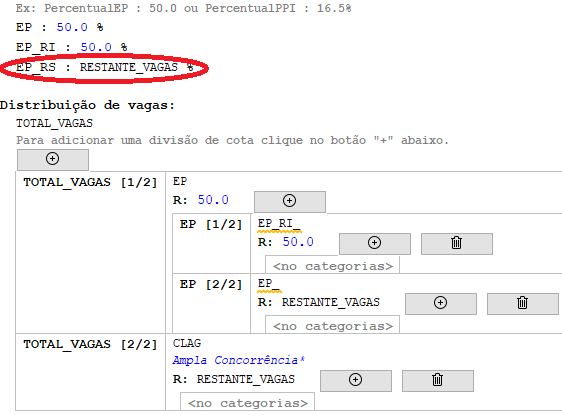
\includegraphics[width=\textwidth]{chapters/analise/imagens/figfalha.png}}

\par\medskip\textbf{Fonte:} Dados da pesquisa (2020). \par\medskip

\end{figure}



\begin{figure}[ht!]
\centering

\caption{\textmd{Problemas na definição da distribuição}}
\label{fig:figerroniveis}
\fcolorbox{gray}{white}{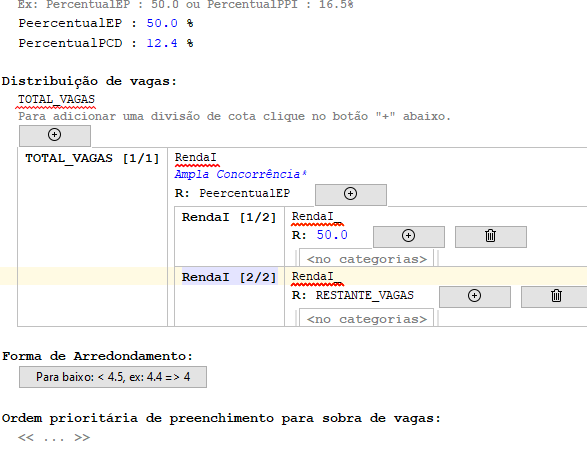
\includegraphics[width=0.85\textwidth]{chapters/analise/imagens/figerroniveis.png}}

\par\medskip\textbf{Fonte:} Dados da pesquisa (2020). \par\medskip

\end{figure}



\newpage
Para o levantamento sobre o grau de dificuldade nas escalas 1 (difícil) até 5 (fácil) observa-se que os Usuários: 2, 6 e 19 apontaram a escala 3, enquanto os usuários 8 e 9 apontaram a escala 4 e 2, respectivamente. O que pode indicar que na maioria dos casos houve dificuldade para entendimento e uso da DSL Cotas.

Em continuidade à análise das dificuldades, consideram-se as seguintes observações dos usuários:

\begin{enumerate}
    \item [a)] "Uma das dificuldades é por ser o primeiro contato com a ferramenta e não ter domínio sobre a mesma. Depois, fiquei com dúvida no preenchimento dos critérios: Eles serão baseados na lei de cotas, ou seja, os percentuais de destinação para cada vaga já estão estabelecidos, fica a critério de quem for criar a árvore a ordem de destino das vagas então? Fiquei com dúvida também se as abreviações deveriam ser conforme o que já consta nos editais e como os inscritos se cadastram no sistema de ingresso, ou se isso não faz diferença. (Usuário 2)"; 
    \item [b)] "Como usuário iniciante, o guia de instruções estava com poucas informações para execução da tarefa. (Usuário 6)";     
    \item [c)] "Como pessoa que não exerce atividade nesse segmento, achei pouco intuitivo. A parte para definição de ordem prioritária, aparentava existirem campos repetidos, pois referente aos alunos RI e RS não encontrei diferenciação entre os 37\% e o restante de vagas (dá a ideia de existirem apenas 3 campos - Alunos RI - Alunos RS - AC). (Usuário 9)";
    \item [d)] "Para organizar as informações no exercício precisei rever o vídeo com as instruções e após a segunda visualização do material com exemplos consegui usar os recursos mais facilmente. (Usuário 19)".     
\end{enumerate}

Desse modo, pontuam-se algumas das dificuldades apresentadas por esse grupo, tais como: dúvidas sobre o preenchimento correto dos percentuais e siglas das categorias (Usuário 2), falta de instruções com passos mais detalhados (Usuário 6), problemas durante a definição das categorias e sua utilização na ordem de prioridade (Usuário 9) e a necessidade de várias consultas no manual e ao vídeo explicativo da DSL (Usuário 19). 

Com relação ao levantamento sobre as deficiências da linguagem, os Usuários 2 e 19 marcaram a opção "O tempo de aprendizagem da linguagem é extenso", enquanto os demais usuários apontaram que "As sugestões das mensagens informativas não são claras o suficiente". 

Em sequência a esse levantamento, os usuários apontaram como comentários e sugestões: 

\begin{enumerate}
    \item [a)] "Achei o sistema em certa medida intuitivo e de fácil manuseio, mas tive dificuldades com o tamanho da fonte das palavras (estava pequeno e não foi possível aumentar usando ctrl+). Acredito que com critérios bem estabelecidos (quais abreviações usar, etc) e um tempo maior de uso a ferramenta será de grande utilidade (Usuário 2)";
    \item[b)] "O guia para 1ª utilização do sistema poderia ser mais detalhado; mensagens de erro poderiam ser exibidas em caixas de texto; tamanho das letras nas caixas de opções, muito pequenas. (Usuário 6)";
    \item[c)] "Nas mensagens de erro ou aviso, constar exemplo correto de preenchimento. (Usuário 8)".   
\end{enumerate}

Por fim, notou-se maior dificuldade de entendimento das mensagens e nos recursos de \textit{feedback} ao usuário, se comparado aos grupos com conhecimento na área de domínio e/ou desenvolvimento de sistemas. Na Subseção \ref{sec:comparativogrupos} é descrito o resumo comparativo entre os grupos analisados.

\subsection{Comparativo entre os grupos de análise}
\label{sec:comparativogrupos}

Em relação aos critérios estabelecidos para a análise, considerando o levantamento apresentado pelas Figuras \ref{fig:quadro:grupodevesp}, \ref{fig:quadro:grupodevnesp}, \ref{fig:quadro:grupondevesp} e \ref{fig:quadro:grupondevnesp}, observou-se que o grupo DEV-ESP teve mais facilidade de entendimento e utilização dos recursos da DSL, uma vez que todos os usuários conseguiram definir as regras propostas pelo exercício, além das soluções apresentarem poucos \textit{errors} e \textit{warnings}. Esse fato reforça que: "o uso de DSLs com entendimento do domínio, deixa o pensamento ser expresso de maneira mais clara quando o código escrito não está repleto de detalhes de implementação"  \cite[p.41, tradução nossa]{dslengineering}.

Em segundo lugar, considerando a correta implementação das regras propostas, no grupo NDEV-ESP apenas 2 (dois) dos 8 (oito) usuários não conseguiram configurar a distribuição completa, no entanto, 6 (seis) usuários fizeram as definições conforme o exercício, sendo que 2 (dois) deles avançaram no desenvolvimento da versão mais recente e complexa da legislação, contemplando candidatos inscritos na categoria PCD. 

O fato dos usuários NDEV-ESP terem conseguido atender uma legislação diferente da proposta, pode se relacionar com um dos benefícios de DSLs: 

\begin{citacao}
O uso de DSLs específicas de domínio, podem parecer, a primeiro momento, difícil de se justificar, porém essas DSLs são normalmente atreladas ao \textit{know-how} do negócio, provendo um meio de descrever conhecimento de maneira formal, organizada e sustentável. \cite[p.43, tradução nossa]{dslengineering}.
\end{citacao}

Em continuidade a esse comparativo, o grupo DEV-NESP ficou em terceiro lugar no que diz respeito ao entendimento sobre os recursos utilizados, esses usuários apontaram no questionário um grau de dificuldade elevado, o que foi agravado pelo fato de desconhecerem a área de domínio. Contudo, apesar das dificuldades, na maioria dos casos, todos os recursos foram utilizados sem que fossem gerados muitos erros ou avisos. 

Por fim, a análise do grupo NDEV-NESP mostra que há potencial de uso da DSL, no entanto, destaca-se que há necessidade de mais explicações sobre as regras de domínio, assim como de capacitação para uso na linguagem. Isso se justifica, pelo fato de que esse grupo apresentou maior quantidade de erros além de alguns exercícios terem sido entregues de forma incompleta.



\subsection{Mudanças resultantes da avaliação}
\label{sec:mudanasresultantes}

Considerando as principais dificuldades relatadas pelos usuários da DSL Cotas, nessa Subseção são descritas as melhorias implementadas na linguagem que foram selecionadas com o objetivo de reduzir as lacunas de entendimento sobre a distribuição das vagas e também melhorar a clareza das mensagens de erros e avisos aos usuários.

A primeira melhoria é a responsável pelo tratamento das sugestões apontados pelos usuários do grupo DEV-ESP e NDEV-ESP, os quais apontaram a necessidade de visualização prévia de simulação das vagas, para tanto foi adicionado um novo elemento do tipo \texttt{behavior}, \texttt{Distribuicao\_Behavior} no qual foram inseridos métodos para varrer a \gls{AST} e fazer os cálculos do quadro de vagas seguindo as definições preenchidas pelo usuário da DSL (Código Fonte \ref{lst:distribuicao_behavior}).

\newpage

\lstinputlisting[language=Java, 
caption=Behavior para cálculo do quadro de vagas 
,label=lst:distribuicao_behavior]{chapters/trechos_codigo/distribuicao_behavior.m}


O método \texttt{calculaDistribuicao} (Linha 3) acessa a \texttt{CategoriaCota} raiz, o valor de simulação desejado e a forma de arredondamento definida pelo usuário, e em sequência, por meio do método recursivo \texttt{calculaVagasCategoria} (Linha 14) são realizadas iterações em todas as categorias subsequentes da distribuição, calculando as vagas conforme os respectivos percentuais (Linha 24) ou fazendo o cálculo de soma das vagas para a constante \texttt{RESTANTE\_VAGAS} (Linha 27). 

Os números de vagas para cada categoria são armazenados em um novo atributo do conceito, nomeado de \texttt{numeroVagas}, esses valores são atualizados sempre que o usuário aciona a função de simulação na DSL ou no caso da forma de arredondamento ser alterada. Desse modo foi possível adicionar novos elementos no editor dos conceitos \texttt{CategoriaCota} e \texttt{Distribuicao} para apresentar o valor calculado, além de gerar uma listagem do quadro de vagas (Figuras \ref{fig:editoralterado}, \ref{fig:simulacaovagas} e \ref{fig:quadrosimulacao}).


\begin{figure}[ht!]
\centering

\caption{\textmd{Editores alterados para simulação de vagas}}
\label{fig:editoralterado}
\fcolorbox{gray}{white}{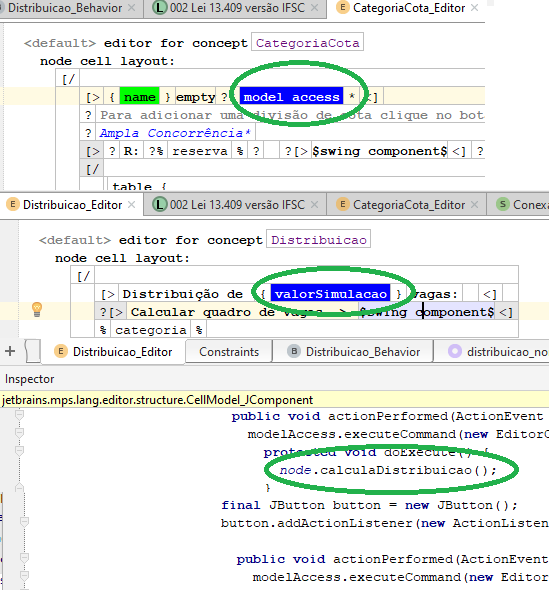
\includegraphics[width=0.65\textwidth]{chapters/analise/imagens/editoralterado.png}}

\par\medskip\textbf{Fonte:} Elaborado pelo autor (2020). \par\medskip

\caption{\textmd{Simulação de vagas durante a definição da distribuição}}
\label{fig:simulacaovagas}
\fcolorbox{gray}{white}{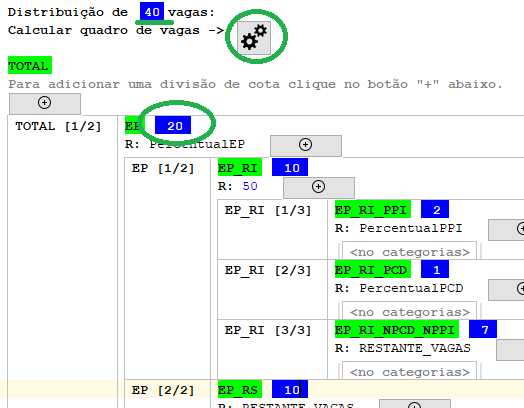
\includegraphics[width=0.75\textwidth]{chapters/analise/imagens/simulacaovagas.png}}

\par\medskip\textbf{Fonte:} Elaborado pelo autor (2020). \par\medskip

\end{figure}



\clearpage
\begin{figure}[ht!]
\centering

\caption{\textmd{Simulação do quadro de vagas}}
\label{fig:quadrosimulacao}
\fcolorbox{gray}{white}{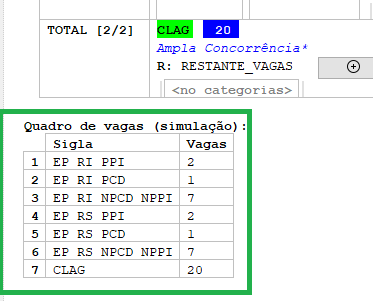
\includegraphics[width=0.55\textwidth]{chapters/analise/imagens/quadrosimulacao.png}}

\par\medskip\textbf{Fonte:} Elaborado pelo autor (2020). \par\medskip

\end{figure}




A visualização prévia dos cálculos pode auxiliar no entendimento dos requisitos de distribuição de vagas para todos os grupos de usuários analisados, possibilitando que tenham uma simulação imediata dos elementos da linguagem, além de auxiliar no caso de dúvidas sobre como os percentuais são aplicados no contexto da árvore de distribuição.

Com relação às dificuldades de entendimento das mensagens de erro e dos avisos apresentados pela linguagem, foram alteradas as instruções para incluir exemplos de formato de preenchimento, além de tratamentos para priorizar as mensagens exibidas de modo que não fossem geradas inconsistências antecipadamente, o que pode contribuir para confundir o usuário sobre o momento correto da sua resolução (Figura \ref{fig:mensagens}).

\begin{figure}[ht!]
\centering

\caption{\textmd{Melhorias nas instruções e mensagens}}
\label{fig:mensagens}
\fcolorbox{gray}{white}{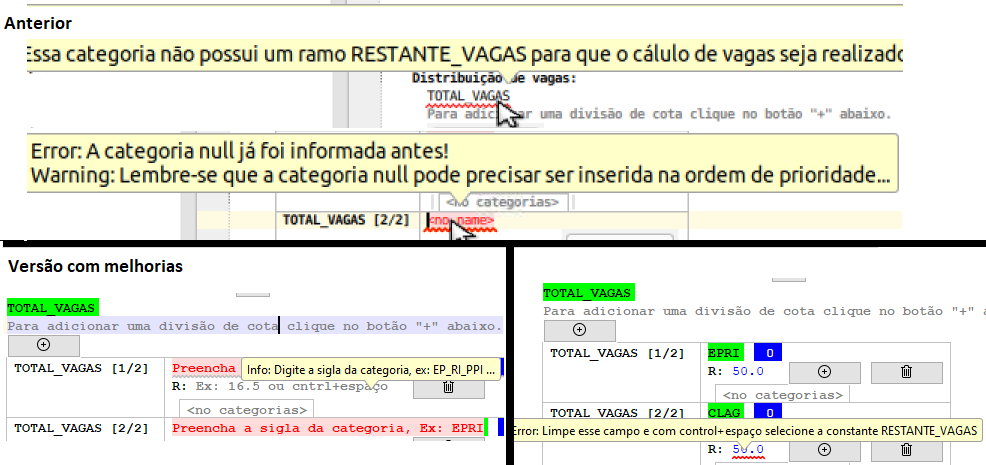
\includegraphics[width=0.94\textwidth]{chapters/analise/imagens/mensagens.png}}

\par\medskip\textbf{Fonte:} Elaborado pelo autor (2020). \par\medskip

\end{figure}



No que diz respeito às dificuldades dos usuários para seleção das categorias na seção \texttt{OrdemPrioridade}, foi alterado o editor dessa seção para permitir adicionar novas categorias por meio do componente \texttt{JButton} o qual facilita a seleção da categoria pelo usuário, sem precisar utilizar apenas o teclado para novas inclusões (Figura \ref{fig:melhoriaordem}). Destaca-se também, a modificação nas mensagens instrutivas sobre o preenchimento da ordem de prioridade, que deixaram de ser apresentadas em cada categoria da árvore de distribuição, para serem requisitadas apenas no momento de definição da ordem de prioridade.

\begin{figure}[ht!]
\centering

\caption{\textmd{Melhorias na seção Ordem de Prioridade}}
\label{fig:melhoriaordem}
\fcolorbox{gray}{white}{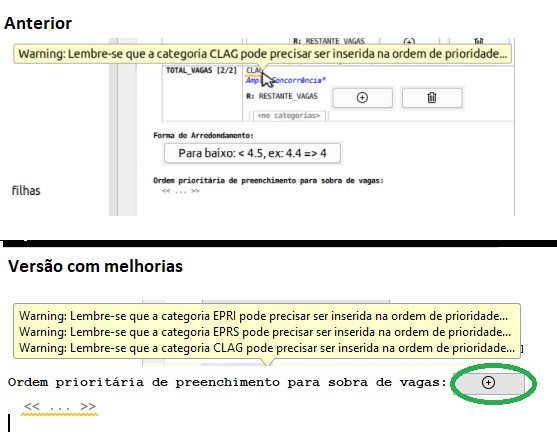
\includegraphics[width=0.94\textwidth]{chapters/analise/imagens/melhoriaordem.png}}

\par\medskip\textbf{Fonte:} Elaborado pelo autor (2020). \par\medskip

\end{figure}



Para tratar as dificuldades relatadas sobre o formato de preenchimento dos percentuais, foi alterada a regra de inferência dos elementos \texttt{Configuracao} e \texttt{CategoriaCota} para aceitar tanto valores inteiros como valores fracionados, evitando que o usuário tenha que preencher por exemplo "50.0". Isso foi possível pela comparação de tipagem fraca (\textit{weak subtype}) ao invés da comparação exata de tipos (\textit{strong subtype}).

\begin{figure}[ht!]
\centering

\caption{\textmd{Regra de inferência com \textit{weak sybtype}}}
\label{fig:weak}
\fcolorbox{gray}{white}{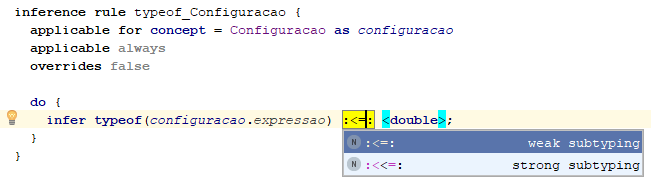
\includegraphics[width=0.75\textwidth]{chapters/analise/imagens/weark.png}}

\par\medskip\textbf{Fonte:} Elaborado pelo autor (2020). \par\medskip

\end{figure}



\newpage
Por fim, as alterações descritas foram realizadas tendo como base as principais dificuldades apontadas pelos usuários da DSL. Desse modo, a versão final pode agregar valor ao presente estudo no que diz respeito ao uso de DSL como ferramenta de melhoria na comunicação entre os envolvidos, reduzindo eventuais incompreensões no uso da linguagem.

Na próxima Seção serão apresentados os resultados da análise com relação aos testes da \gls{API} DSL Cotas.

\section{Resultados obtidos com a API DSL Cotas}
\label{sec:avaliacaoapi}

Nessa Seção são descritos os resultados provenientes dos testes da API DSL Cotas, nos quais tiveram como objetivo principal a comparação do histórico de processos seletivos do \gls{IFSC} com o resultado gerado pela API, de modo a verificar a conformidade de seus resultados em relação às legislações vigentes e/ou mais antigas.

Essa análise contou com a seleção aleatória de 16 processos seletivos, incluindo 403 cursos do tipo: técnico integrado, concomitante, subsequente, proeja e graduação. Nesse contexto, foram considerados os resultados de 13494 candidatos no período de 2013 até 2020, nos quais foi possível testar 2 (duas) das versões já processadas pelo sistema de ingresso, além das demais alterações de código ocorridas no período. 

Não foi possível fazer o comparativo com a versão intermediária descrita na Subseção \ref{versao2} do Capítulo \ref{chap:historicoversoes}, uma vez que não houve processamento de resultados na época, pois o código precisou ser atualizado com a versão mais recente disponibilizada pelo MEC, antes da sua utilização nos processos seletivos.

Como resultado dos testes foi gerado um relatório contendo as colunas, "Versão de lei utilizada", "Edital", "Identificador do Curso", "Número de vagas", "Código de Inscrição", "Classificação", "Categoria esperada" e "Resultado da conferência". Para cada candidato foi acionado o \textit{endpoint} \texttt{aprovaCandidatos} em classe de testes do \texttt{JUnit}, na qual foram realizadas requisições \texttt{HTTP} passando a lista de inicial de candidatos inscritos, sem a situação de classificação.

A listagem resultante da API passou por comparação de todas as siglas de situação de classificação conforme o sistema de cotas, sendo possível retornar e comparar a sigla de situação original presente na base do sistema de ingresso. Desse modo, foi verificado que 81 dos 403 cursos apresentaram divergências nas listas de classificação de candidatos.

Essas divergências foram marcadas em 297 candidatos dos 13494 registros utilizados. Para cada curso com divergência foi realizada uma análise manual que teve como objetivo identificar o problema, o motivo e uma possível solução. Essas divergências foram agrupadas nas seguintes \textit{issues} cadastradas no repositório \texttt{https://github.com/estrazulas/dsl-cotas-gen/issues}:

\begin{enumerate}
    \item[a)] \textbf{Candidato sem situação de classificação}: Situação encontrada em 2 (dois) cursos, o problema apresenta alguns candidatos sem sigla de categoria na lista resultante com o uso da API. Nos 2 (dois) casos, o motivo da divergência aponta para o fato de o teste ter sido realizado apenas em candidatos de primeira chamada, sendo que os candidatos com problema foram convocados posteriormente pelo sistema de ingresso. Não sendo um problema a ser solucionado pela API, uma vez que em chamadas posteriores as situações seriam recalculadas;
    
    \item[b)] \textbf{Cursos com candidatos em rechamada}: Em 31 dos cursos testados foram encontrados candidatos em situação de inscrição "REC" ou re-chamados, no entanto, a seleção de candidatos para aplicação do testes apenas considerou a busca por candidatos de primeira chamada e em situação "CLA", sigla utilizada antes da etapa de aprovação e atribuição de categorias. Os candidatos re-chamados faziam parte de uma regra de negócio antiga do sistema, que dava a oportunidade de serem reconvocados para matrícula em chamadas posteriores, e por esse motivo não entraram no filtro de comparação de candidatos em primeira chamada;
    
    \item[c)] \textbf{Candidato cotista convocado como ampla concorrência}: Em apenas um curso foi encontrado um candidato de inscrição por cotas que na API foi marcado para a categoria correta, no entanto, no sistema de ingresso consta com a categoria de ampla concorrência. Após análise manual identificou-se que seguindo as regras de processamento, o candidato da posição 18 deveria ter sido convocado como cotista. No entanto, a causa dessa divergência é desconhecida, sendo possível que na época esse candidato tenha sido alterado manualmente em base de dados;
    
      
    \item[d)] \textbf{Candidato da ampla concorrência classificado como cotista}: A divergência com maior número de casos (42 cursos do \gls{SISU}). Após análise no processamento foi identificado que os candidatos inscritos como cotistas com pontuação superior aos de candidatos da ampla concorrência (CLAG) foram aprovados pelo \gls{SISU} como cotistas, quando em todos os demais processos seletivos do sistema o funcionamento sugere que os primeiros colocados sejam selecionados e classificados pela categoria CLAG. Em síntese, o processamento foi diferente ao adotado pelo SISU, o que não pode ser resolvido no contexto da presente pesquisa.
    
\end{enumerate}

Destaca-se que as divergências encontradas foram provenientes de situações ocorridas durante o andamento dos processos de inscrições de candidatos, não sendo possíveis de serem tratadas pela DSL Cotas, uma vez que o próprio sistema de ingresso modificou as situações de classificações na medida em que outras chamadas foram sendo realizadas.

Nos demais casos de divergência foram identificados candidatos com problemas relacionados a operações na base de dados em função de abertura de chamados do setor demandante, ou situações que puderam ser identificadas e resolvidas por meio de correção do código da API. O detalhamento completo das divergências, assim como o relatório utilizado para a análise estão disponíveis no repositório \textit{github} citado anteriormente.

Por fim, essa análise sugere que na maioria dos casos de cursos testados foi possível combinar o formalismo definido pela DSL Cotas em conjunto com a API, de modo a validar os diferentes tipos de cursos e versões da legislação já utilizadas pelo \gls{IFSC}. A sua utilização pode favorecer a produtividade e a evolução de novas alterações em lei, de maneira agnóstica sem estar atrelada a uma \gls{GPL} específica, uma vez que sua construção foi concebida a nível de serviços \textit{web}.




